\section{Introduction}

This essay argues for the moral permissibility of introducing hyper-tracing, which is a proposal that has been widely discussed during the Covid-19 pandemic.
However, it is easy to see that moral permissibility highly depends on when this discussion takes place.
Certainly years after the disease is eradicated, it is unfounded to consider the introduction of hyper-tracing.
During the pandemic, the moral permissibility of such action is, however, not clear.

This essay is written from the perspective of the state of the world and the knowledge of early 2020. The rationale for this is that the future development of this pandemic was the most uncertain at this point..\footnote{There were only vague predictions on how fast the cure could be developed and distributed, how the pandemic will spread and the testing was expensive and unorganized.}
As such, many new measures were introduced during this month (most notably lockdowns and mandatory masks) and hyper-tracing was also part of the discussion.
The soundness of the argument relies upon this consideration - namely the truthfulness of one of the premises.

\section{Main Argument}

The main argument of this essay in favour of hyper-tracing is based on the presence of a global pandemic making the gain of the introduction of such a measure higher than the burden.
It is also argued that other solutions which could drastically affect the situation for the better either do not exist or have even higher burdens.

The top-level argument is sketched in extended standard form in \Cref{subsec:esf}, its validity verified in \Cref{subsec:logical} and the truthfulness for the individual premises discussed in \Cref{subsec:premises}.
Namely, the given reasons for believing premise P8 provides an overview and rationale for the rest of the argument.

\subsection{Extended Standard Form} \label{subsec:esf}

\begin{argument}
    \premise{P1}{Hyper-tracing is a measure that provides information to the authorities about proximity contact of most of the people and whether they have been tested, infected, quarantined or vaccinated.}
    \premise{P2}{If a hyper-tracing provides the information to the authorities about the proximity contact of most of the people and whether they have been tested, infected, quarantined or vaccinated then it leads to the authorities being able to issue recommendations for testings or quarantines.}
    \premise{P3}{If hyper-tracing leads to the authorities being able to issue recommendations for testings or quarantines then hyper-tracing leads to outbreaks being significantly reduced.}
    \premise{P4}{If hyper-tracing leads to significantly decreasing the number of outbreaks then it is a solution for the pandemic.}
    \intermediate{C1}{Hyper-tracing is a measure that is a solution for the pandemic.}{P1-4}
    \premise{P5}{
    There is a global pandemic.}
    \premise{P6}{
    If there is a global pandemic, then the burden of introducing hyper-tracing is less than the gain.}
    \intermediate{C2}{The burden of introducing hyper-tracing is less than the gain.}{P5-6}
    \premise{P7}{Other known measures other than hyper-tracing cause either more significant burden or are not solutions for the pandemic.}
    \premise{P8}{
    If the burden of a measure that is a solution for the pandemic is less than the gain and other known measures are either not solutions for the pandemic or cause significantly more burden than the gain then the action is morally permitted.}
	\conclusion{C}{It is morally permitted to introduce hyper-tracing.}{C1, C2, P7, P8}
\end{argument}

\subsection{Logical Form} \label{subsec:logical}

From solely predicate logic the main argument is not valid since P4 and P7 are general statements about all actions and therefore part of the premise in P7 is different from the conclusion of P6.

Rewriting the argument in first-order logic makes it clear that the argument is valid. The sentence of P7 ($O(h)$) could be expanded to $\forall x: x \ne h \rightarrow (\neg BG(x) \vee \neg S(x))$ though since the inner structure is not used in the rest of the argument, it is denoted as $O(h)$ for simplicity. Predicate translations are clear from the extended standard form.

\begin{argument}
    \premise{P1}{$M(h) \wedge PI(h)$}
    \premise{P2}{$PI(h) \rightarrow AITQ(h)$}
    \premise{P3}{$AITQ(h) \rightarrow HSD(h)$}
    \premise{P4}{$HSD(h) \rightarrow S(h)$}
    \premise{C1}{$S(h)$}
    \premise{P5}{$P$}
    \premise{P6}{$P \rightarrow BG(h)$}
    \premise{C2}{$BG(h)$}
    \premise{P7}{$O(h)$}
    \premise{P8}{$\forall y: (BG(y) \wedge S(y) \wedge O(y)) \rightarrow MP(y)$}
	\conclusionSimple{C}{$MP(h)$}{}
\end{argument}

The usage of implication in P4 is somewhat inaccurate because it does not capture the full meaning of \emph{because}. It would be trivially true if the middle predicate was something true but completely unrelated to the condition which would make the measure a solution even though that is not what people would infer intuitively from the original sentence. In this case, the causality is clear.

By instantiation of the quantified variable in P8 as $y=h$, the validity of the argument is clear.

\subsection{Reasons to Believe the Premises} \label{subsec:premises}

\subsubsection*{P1}

The truthfulness of this premise clearly follows from the description of hyper-tracing in the instructions.

\subsubsection*{P2}

Following the reasoning from the description, having information about possible contacts and infections makes it possible for the authorities to issue recommendations for testing or quarantine.

\subsubsection*{P3}

The information about possible contacts and infections makes it easier to plan vaccination distribution and obviously to also issue quarantine recommendations to those who may have been in contact with an infected person. 
This vastly reduces the number of unconscious carriers which in turn helps in significantly decreasing the number of outbreaks.

\subsubsection*{P4}

It is clear that if disease outbreaks are prevented, then the disease spreads much more slowly and therefore anything that prevents disease outbreaks is a possible solution to the pandemic.

\subsubsection*{P5}

It is clear that from the perspective of this essay (early 2020), there was an unmanaged ongoing global pandemic, Covid-19.

\subsubsection*{P6}

The gains from hyper-tracing are mostly the reasons why it is a solution.
However, that may not be the only source of gains and burdens and therefore it is necessary to argue separately why overall the gains outweigh the burdens.

% Obviously, all the gains and burdens are conditioned on there being a global pandemic.
The biggest gain is that the introduction saves lives because it gets the number of infections down (formal argument for this is P1-4).
This is highly desirable from most philosophical perspectives\footnote{Deontological ethics is the most straightforward though most axiologies for consequentialism would surely rate preventing human deaths very high.} as it appears to be universal to want to save as many human lives as possible.

For burdens, it is clear it violates privacy, specifically data protection, making it a privacy threat.
This is because that an individual no longer has enough auditing power to examine the whole process to determine whether the data is being misused.
Lastly, it implements a tool that could potentially be used for government purposes other than those related to pandemic handling.
Although this would not be enough to enable a police state, it would be one of the tools that would make the change easier.
Such increased threat is undesirable because of oppression, limited freedom and general lack of autonomy.

On a larger scale, the introduction ensures that normal life is possible.
This can be motivated by the re-gained autonomy and being allowed to fully participate in the economy again (preference satisfaction).
On the other hand, there may be a view in which it is not desirable to return to the ,,normal life'' and that the current situation offers more benefits.
These include: (1) lower pollution and resource exploitation due to restricted economic activity, (2) potential for reconstruction of halted sectors (infrastructure, industry, food supplies etc) or (3) spending less time commuting (assuming lockdown would be implemented instead).

Overall, saving a large number of preventable deaths and returning to ,,normal life'' is weighted against a mild privacy violation and providing tools that could be misused in the future for implementing a totalitarian government.
The threat of enabling a totalitarian government is however not palpable and there are multiple other tools that would help prevent it.
A mild privacy violation, albeit a real burden, can be outweighed by preventing human deaths.

\subsubsection*{P7}

This premise states that of all known solutions to the pandemic, this one bears the least burden compared to the gains.
The gains and not solely the least burden should be considered since there may be some solutions that only partially improve the situation (qualifying to be called a solution) which would mean that they would have little burden but would also offer very little gain.

% This premise is complicated in two ways: (1) what we measure as burdens and gains depend heavily on the philosophical framework we choose and (2) the set of possible known measures is very diverse and possibly infinite (due to parametrization) and therefore proving the optimality of single one is not straightforward.
% This premise is complicated by the set of possible known measures being very diverse and possibly infinite (due to parametrization).
% Therefore proving the optimality of a single one is not straightforward.

Despite the set of possible known measures is possibly infinite due to parametrization, I consider the following alternative solutions since they were the most discussed:\footnote{I do not consider voluntary tracing because as the pandemic showed, it was not adopted enough for it to become a solution.} lockdowns and mandatory testing.
A combination of the two could obviously be implemented, though by showing that each of the two measures has a higher burden than the gains, I can assume that their combination would also have the same properties.
There are of course many other measures that would technically qualify as solutions, like preemptively killing off susceptible people, though I filter them because of their absurdity and clearly high burdens compared to gains.
% With all measures, we also assume the basic measure of mask mandates and distancing, which does not create a significant burden for most people and has shown to be systematically helpful, though not a solution by itself.

By \emph{lockdowns} I understand a state-wide law forbidding non-essential travel and high restrictions on movement outside one's own home.
As a result, most stores and most of the service and hospitality sector would be closed as well.
Similar to P6, the gain is the saving of human lives.
The burdens include very serious infringement of autonomy in the form of movement because it would no longer be possible to freely assemble or to move unrestricted.
It also hinders other desirable values, such as pursue of education.
Other, less significant burdens would include health issues (mental and physical) developed in prolonged staying in one place and an increase in domestic abuse.
Since the gains of lockdowns and hyper-tracing mostly align with saving human lives, their burdens can be compared.
A privacy violation appears then to be less of a burden than losing the freedom of movement which is more imminent than the malicious actions that could arise from the misuse of hyper-tracing.

By \emph{mandatory testing} I mean a large-scale organization of regular testing for everyone.
It is unclear whether this would be implementable state-wide because of the logistic issues and the cost of such testing.
Assuming it would be possible, the gains would be the immediate knowledge of new infections and being able to act quickly upon it (quarantines).
This would lead to the most significant gain, preventing outbreaks and therefore saving human lives.
The burdens however include very large economic costs for running such an operation (both the organization and the material).
Requiring everyone to get tested, e.g. every two days would be an inconvenience for everyone.
It would also significantly reduce one's autonomy by forcing the actual testing and also requiring everyone to move to the testing location.
Such an organization system would also require a centralized registry so that it can report whenever anyone did not show up for testing.
This could be implemented in such a way that it does not log from which testing centre the testing comes from, though this would remain a privacy threat.
In comparison to the burdens of hyper-tracing, I am weighting a privacy violation against a privacy threat, autonomy restriction, inconvenience for every citizen and a significant economic cost.
Although there is no single deciding factor in the burdens of mandatory testing, overall they seem to outweigh the single significant burden of hyper-tracing.

Note that having a developed vaccine and the capacity for distribution would obviously impose much less burden than any other solution.
This would be true even without actually having the vaccine but with the prospect of it in the future.
Around early 2020, this was, however, still not true.

\subsubsection*{P8}

This premise stems from the fact that I am looking for the best measure among all suitable solutions.
The formula states that if a given measure fulfils the following three conditions, then it is morally permitted to introduce that measure.
The conditions are:

\begin{itemize}[noitemsep]
\item The measure is a solution for the pandemic.
\item Burden of introducing the measure is less than the gain.
\item Other known measures are either not a solution for the pandemic or the burden of introducing them is higher than the gain.
\end{itemize}

The rationale for the first item is clear.
If a given measure does not provide a solution for the pandemic, then it can not be justified on the grounds of us looking for the best solution.\footnote{The implication form of the statement allows for it to still be justifiable for different reasons.}
% It does not mean that it is not morally justifiable.

The second item filters out measures that would even perhaps be solutions but with too significant burdens that outweigh the gains.
An example of this would be killing everyone on Earth.
This would reduce the number of outbreaks but obviously at an absurdly high burden.

Lastly, I am interested in the best measure of the set of measures that are solutions and which have only reasonable burdens compared to the gains.

\section{Attack}

\subsection{Attacking a Premise}

The most promising attack is to examine P8.
It is based on generally believable premise that the best of all possible actions is necessarily also the morally permissible one.
This is appealing and based on Kant's \emph{should implies can}.
If everyone is required to do only morally permissible actions, then certainly there must be at least one morally permissible action in the set of actions they can do that is morally permissible.
Premise P8 is implicitly built on this premise though it reduces the set of all actions to measures that are solutions to the pandemic.
The reduction to measures does not bear much semantic meaning and as such is not problematic (simply names for actions that are decided on government-level; it is not required to be a policy that is needed to be introduced) though the reduction to solutions is. 

It disallows measures that are not solutions though are relevant to the handling of the pandemic to be permissible.
Namely, this results for such measures (i.e. requiring only masks and distancing) to not be compared with possible solutions to the pandemic, making them easier to defend.
Just because other solutions to the pandemic are worse does not mean that it is morally permissible to introduce the best one.\footnote{This would be the case with all measures but not necessarily with the set of solutions to the pandemic.}
There may be other measures, not solutions, which would be overall the best measure, making them morally permissible on the grounds of the best possible action being the moral permissible one.

\begin{argument}
\premise{P1'}{In some situations the set of morally permissible solutions to the pandemic with higher gains than burdens can be empty.}
\premise{P2'}{
    If
    \emph{in some situations the set of morally permissible solutions to the pandemic with higher gains than burdens can be empty}
    then
    \emph{in some situations in which a solution that has higher gains than burdens and is better than all other solutions is not morally permissible.}
}
\premise{P3'}{
    If
    \emph{it is plausible that there are situations in which a solution which has higher gains than burdens and is better than all other solutions is not morally permissible}
    then it is not the case that
    \emph{if the burden of a measure that is a solution for the pandemic is less than the gain and other known measures are either not solutions for the pandemic or cause significantly more burden than the gain then the action is morally permitted.}}
\conclusion{C'{\footnotesize =$\neg$P8}}{
    It is not the case that \emph{if the burden of a measure that is a solution for the pandemic is less than the gain and other known measures are either not solutions for the pandemic or cause significantly more burden than the gain then the action is morally permitted.}
}{P1'-3'}
\end{argument}

\subsection{Defense}

I start with a premise that follows from Kant's statement, that the set of morally permissible measures is non-empty (P1'').

I follow with a premise that the set of morally permissible measures to the pandemic is empty (P2'').
This is motivated by the fact that in most societies, preventable human deaths are a very high priority which outweighs economic and cultural plans, therefore any measure that is not a solution would not be morally permissible.

Clearly, the set of measures with burdens overweighing the gains does not contain a morally permissible measure (P3'').

From this follows that there is a morally permissible action that is part of the set of measures that are solutions and have higher gains than burdens (P4'').
From this set, I am taking the best one, which must be morally permissible.

\begin{argument}
\premise{P1''}{$\{m|MP(m)\} \neq \emptyset$}
\premise{P2''}{$\{m|MP(m) \wedge \neg S(m)\} = \emptyset$}
\premise{P3''}{$\{m|MP(m) \wedge \neg BG(m)\} = \emptyset$}
\premise{P4''}{$(\{m|MP(m) \wedge \neg S(m)\} = \emptyset \wedge \{m|MP(m) \wedge \neg S(m)\} = \emptyset) \rightarrow \{m|MP(m) \wedge S(m) \wedge BG(m)\} \neq \emptyset$}
\intermediate{C1''}{
$(\{m|MP(m) \wedge S(m) \wedge BG(m)\} \neq \emptyset)$
}{P1''-4''}

\premise{P5''}{
$(\{m|MP(m) \wedge S(m) \wedge BG(m)\} \neq \emptyset) \rightarrow$
\newline
$(\forall y: (BG(y) \wedge S(y) \wedge O(y)) \rightarrow MP(y))$}
\conclusion{C''{\footnotesize =P8}}{$\forall y: (BG(y) \wedge S(y) \wedge O(y)) \rightarrow MP(y)$}{C1'', P5''}
\end{argument}

The argument is provided in the logical form for clarity and
shown in \Cref{fig:venn}.

\begin{figure}[h!]
\center
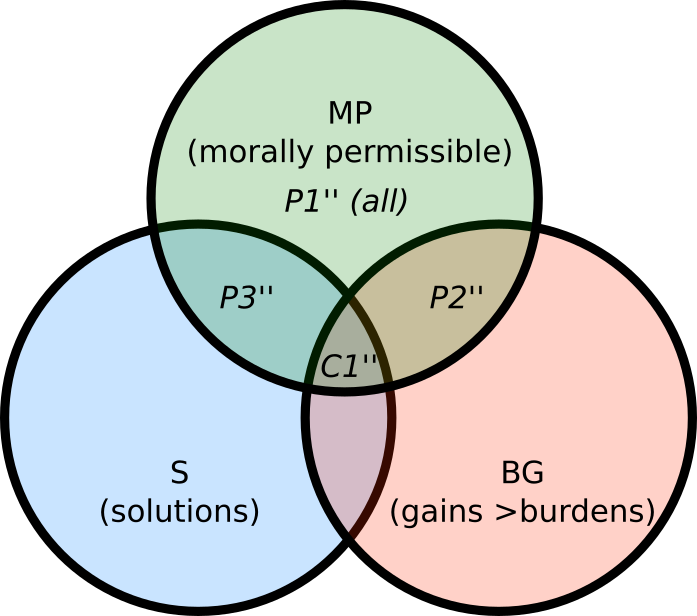
\includegraphics[width=0.45\linewidth]{img/venn.png}
\caption{Illustration of sets relevant in the defense. Premise names in italics denote which premise asserts that that region is (non-)empty.}
\label{fig:venn}
\end{figure}

% An alternative would be to add a premise that shows that there exists at least one solution to the pandemic which has higher gains than burdens.
% This would directly show the truthfulness of C1''.

\section{Conclusion}

In this essay, I showed arguments for the introduction of hyper-tracing being morally permissible.
The main argument consisted of the need of having to find a solution because saving a large number of human lives seems to be universally important.
The search then becomes focused on finding the solution where the gains outweigh the burdens the most. 
In this context, I examined hyper-tracing in comparison to lockdowns and large-scale mandatory testing and saw that the burdens are less than the two other alternatives.

The most promising attack seemed to be to disprove that there must exist at least one solution to the pandemic with higher gains than burdens.
This premise is, however, not hard to justify by making inferences using sets and adding two notable premises (1) there exists at least one morally permissible measure and (2) that there does not exist a measure that is not a solution that would be morally permissible.